\section{VIM学习笔记}

\subsection{删除不符合指定格式的行}
当需要删除不符合指定格式的行时,需要命令, 保留\emphasizebox{RES = }, 指令格式:
\begin{messagebox}
:v/RES = /d
\end{messagebox}

\subsection{删除文件中的\^M 符号}
\^M是windos的dos文件格式特有的换行符,在linux上你可以通过cat -A 文件名看到这些隐藏字符。当您的文件是dos格式时,就会出现这个\^M.所以一些shell脚本执行就会出现莫名其妙的问题, 解决方法:
\begin{itemize}
\item vi filename打开文件,执行:set ff=unix 设置文件为unix,然后执行:wq,保存成unix格式。
\item 批量删除命令:
\begin{messagebox}
:%s/\r//g
\end{messagebox}
\end{itemize}

\subsection{VIM分屏命令}
\begin{itemize}
\item 水平分屏
\begin{messagebox}
:split [FILENAME]
:sp [FILENAME]
\end{messagebox}
\item 垂直分屏
\begin{messagebox}
:vsplit [FILENAME]
:vs [FILENAME]
\end{messagebox}
\end{itemize}

\subsection{GVIM修改配置}
\begin{itemize}
\item 开启循环搜索,注释掉:
\begin{messagebox}
"set nowrapscan              " 禁止在搜索到文件两端时重新搜索
\end{messagebox}

\item 取消c语法高亮问题:
\begin{messagebox}
" ~~~C语言语法高亮
let g:std_c_en = 0
if (g:std_c_en)
Bundle 'vim-scripts/std_c.zip'
endif
\end{messagebox}

\item 解决高亮当前词跳到下一个问题:
\begin{messagebox}
nmap fd *''N
\end{messagebox}

\item 解决注释快捷键问题:
\begin{messagebox}
" ~~~注释与反注释所选内容(两个插件可以二选一)
let g:tcomment_en = 1
if (g:tcomment_en)
Bundle 'vim-scripts/tComment'
Bundle 'scrooloose/nerdcommenter' "打开该行
endif
"NERDCommenter注释快捷键
vmap // <leader>ci
\end{messagebox}

\item 解决复制粘贴问题:
\begin{messagebox}
set clipboard=unnamed
\end{messagebox}

\subsection{vim backspace问题}
在xshell中配置如下:
%\begin{figure}[ht]
\begin{figure}[H]
\centering
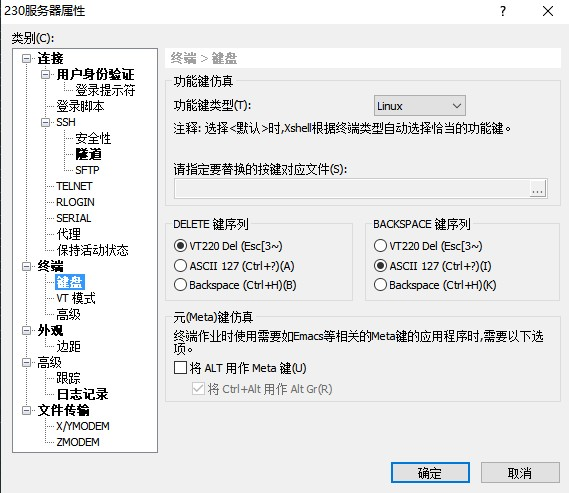
\includegraphics[scale=0.7]{vim_backspace1.jpg} %下划线不用斜杠
%\caption{建立项目}
\label{fig:createproject}
\end{figure}

%\begin{figure}[ht]
\begin{figure}[H]
\centering
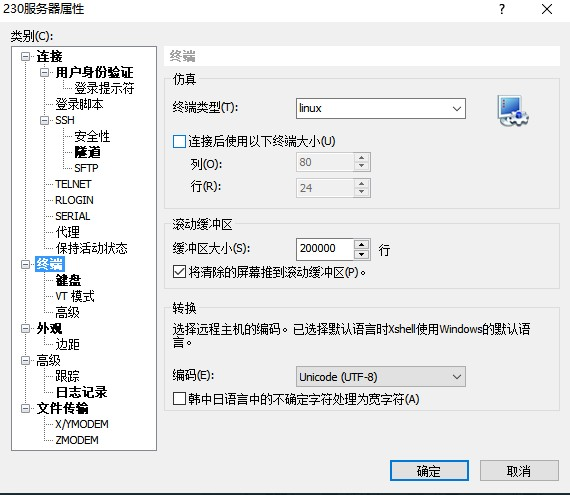
\includegraphics[scale=0.7]{vim_backspace2.jpg} %下划线不用斜杠
%\caption{建立项目}
\label{fig:createproject}
\end{figure}


\end{itemize}
